\documentclass[10pt]{article}
\usepackage[margin=1in]{geometry}
\usepackage{amsmath,amssymb,booktabs,graphicx,hyperref,microtype}
\usepackage[numbers,sort&compress]{natbib}
\newcommand{\RFS}{\textsc{RFS}}
\newcommand{\E}{\mathbb{E}}
\title{Root-Free Shampoo at 125M Parameters:\\A Controlled MI300X Study on One Billion FineWeb-Edu Tokens}
\author{Anonymous}
\date{}

\begin{document}
\maketitle

\begin{abstract}
I evaluate Root-Free Shampoo (\RFS), an eigendecomposition-free realization of
Shampoo's inverse fourth-root preconditioner, on a 124.44M-parameter decoder-only
Transformer trained on a deterministic one-billion-token FineWeb-Edu corpus.  The
study compares AdamW, Shampoo, SOAP, and \RFS under a shared model, data order,
token budget, precision policy, and hardware stack.  I tune each optimizer in a
budgeted two-stage sweep and then run three independent seeds per method.  In
addition to held-out loss, I report end-to-end wall time, optimizer latency,
throughput, memory, power, and the defining \RFS{} numerical certificate.  The
artifact includes native HIP/C++ kernels specialized for AMD's gfx942 architecture
and fully reproducible data manifests, configurations, logs, and analysis code.
\end{abstract}

\section{Introduction}
Adaptive first-order optimizers are inexpensive but discard correlations between
coordinates. Shampoo instead accumulates Kronecker factors and preconditions a
matrix gradient on both sides~\citep{gupta2018shampoo}. Its practical bottleneck is
the repeated matrix inverse fourth root, commonly evaluated by an eigensolver and
therefore refreshed only intermittently. SOAP tracks Shampoo eigenbases while
running Adam in the rotated coordinates~\citep{vyas2024soap}. \RFS{} asks a narrower
question: can the same dense Shampoo operator be realized without an eigendecomposition
using only matrix multiplications and certified iterations?

This paper is an empirical systems study rather than a claim that every workload
favors second-order optimization. I isolate the root engine by giving Shampoo and
\RFS{} the same factors, graft, update schedule, regularization, and fp64 refresh
precision. I also include AdamW~\citep{loshchilov2019adamw} and the authors' SOAP
state-transition rules as external baselines. Every final conclusion is based on
three seeds after optimizer-specific tuning.

\section{Root-Free Shampoo}
For a matrix parameter $W_t\in\mathbb{R}^{m\times n}$ with gradient $G_t$, the
exponential-factor form used here is
\begin{align}
 L_t &= \beta L_{t-1} + (1-\beta)G_tG_t^\top/n,\\
 R_t &= \beta R_{t-1} + (1-\beta)G_t^\top G_t/m,\\
 \widetilde G_t &= L_t^{-1/4}M_tR_t^{-1/4},
\end{align}
where $M_t$ is the bias-corrected first moment. I apply Adam grafting: the
preconditioned direction is rescaled to the norm of the corresponding Adam update.
This controls step magnitude and makes the comparison primarily about direction.

\subsection{Coupled Newton--Schulz RFS}
Let $A=L/\lVert L\rVert_F$. Its spectrum lies in $(0,1]$. A coupled
Newton--Schulz iteration computes a square root and inverse square root without an
eigendecomposition:
\begin{align}
Y_0=A,\quad Z_0=I,\qquad
T_k&=\tfrac12(3I-Z_kY_k),\\
Y_{k+1}&=\operatorname{sym}(Y_kT_k),&
Z_{k+1}&=\operatorname{sym}(T_kZ_k).
\end{align}
In exact arithmetic, $Y_k\rightarrow A^{1/2}$ and
$Z_k\rightarrow A^{-1/2}$. I apply the construction twice: first to obtain
$B=A^{1/2}$ and then to obtain $(B/\lVert B\rVert_F)^{-1/2}$. Restoring both
normalizations yields $X=L^{-1/4}$. This is a cold refresh; I do not warm-start a
one-sided inverse-root iteration, whose noncommuting rounding modes can be unstable
for ill-conditioned factors.

The implementation stops each matrix independently when the coupled residual reaches
$50\epsilon_{\mathrm{mach}}$ or ceases to improve meaningfully for four iterations
after entering the numerical floor. The online certificate is
\begin{equation}
  c(X,L)=\frac{\lVert X^4L-I\rVert_F}{\sqrt{\dim L}}.
\end{equation}
Early language-model gradients make nearly rank-deficient factors. I therefore use
scale-relative regularization $L+10^{-3}\operatorname{tr}(L)I/n$ and evaluate both
\RFS{} and the Shampoo eigensolver in fp64 before casting the preconditioner to fp32.
This precision choice is held fixed across the two methods.

\subsection{Why ``root-free''}
The name denotes removal of an explicit spectral root primitive, not removal of the
mathematical operator. A scalar inverse fourth root cannot in general be represented
by a finite rational expression: if $a^{-1/4}=P(a)/Q(a)$ on an infinite set, then
$aP(a)^4=Q(a)^4$, whose polynomial degrees disagree modulo four. Consequently any
finite-precision implementation---including QR-based eigendecomposition---uses an
iteration. \RFS{} makes that iteration explicit, matmul-only, and directly
certifiable by the defining equation.

\section{Experimental design}
\paragraph{Model.}
The decoder has 12 layers, width 768, 12 attention heads, context length 1024,
GELU MLP expansion four, learned positions, tied GPT-2 token embeddings, and
124,439,808 trainable parameters. Residual projections use the GPT-2 scaled
initialization~\citep{radford2019gpt2}. Forward and backward matrix operations use
BF16; logits are promoted to fp32 for cross-entropy.

\paragraph{Data.}
I tokenize FineWeb-Edu~\citep{penedo2024fineweb} from Hugging Face's pinned
\texttt{HuggingFaceFW/fineweb-edu} sample-10BT
revision with the GPT-2 tokenizer. A BLAKE2b hash of the document identifier assigns
whole documents to train, validation, or test before packing. Exact quotas are
998M/1M/1M tokens. The manifests include SHA-256 digests. Fixed batch geometry
processes 997,720,064 training tokens per nominal one-billion-token run; the small
remainder is reported rather than silently changing sequence or optimizer-batch
shape.

\paragraph{Optimizers and selection.}
The candidates are AdamW, dense Shampoo with Adam grafting, SOAP, and \RFS{} with
the same grafting implementation as Shampoo. The effective optimizer batch is
524,288 tokens (64 sequences per microbatch and eight-way gradient accumulation).
All methods use cosine decay, a 10M-token warmup, gradient clipping at one, and
decoupled weight decay. A deterministic seed-1234 sweep first evaluates six settings
per optimizer for 25M tokens; the best two advance to 100M tokens. Selection uses
validation cross-entropy only. I then evaluate the selected setting at seeds 1, 2,
and 3. Optimizer order rotates by seed to reduce correlation with server age and
temperature.

\paragraph{Hardware and cost.}
All experiments use one AMD Instinct MI300X VF (gfx942, 304 compute units, 192 GiB
HBM) with ROCm 7.14 and PyTorch 2.12 in a pinned container. The host exposes 20 CPU
cores and 235 GiB RAM. Rental cost is integrated by timestamp at \$2/hour through
July 31, 2026 and \$2.50/hour from August 1, with a \$75 absolute ceiling. Dataset
preparation, compilation, pilots, sweeps, final runs, and analysis are included in
the continuous-server ledger.

\paragraph{Native kernels.}
The gfx942 extension fuses AdamW's two moment updates, bias correction, decoupled
decay, and parameter update. Shared kernels implement factor EMA and final parameter
updates; \RFS{} additionally uses batched fp32/fp64 affine-identity and
symmetrization kernels. Large GEMMs use rocBLAS and Shampoo roots use rocSOLVER. Every
native primitive is parity-tested before long runs.

\section{Results}
Figure~\ref{fig:curves} reports seed means and one standard deviation for training
and validation loss. Table~\ref{tab:results} reports the held-out and systems
outcomes. Wall time is end-to-end and includes periodic evaluation, optimizer cold
start, refreshes, and final test evaluation.

\begin{figure}[t]
  \centering
  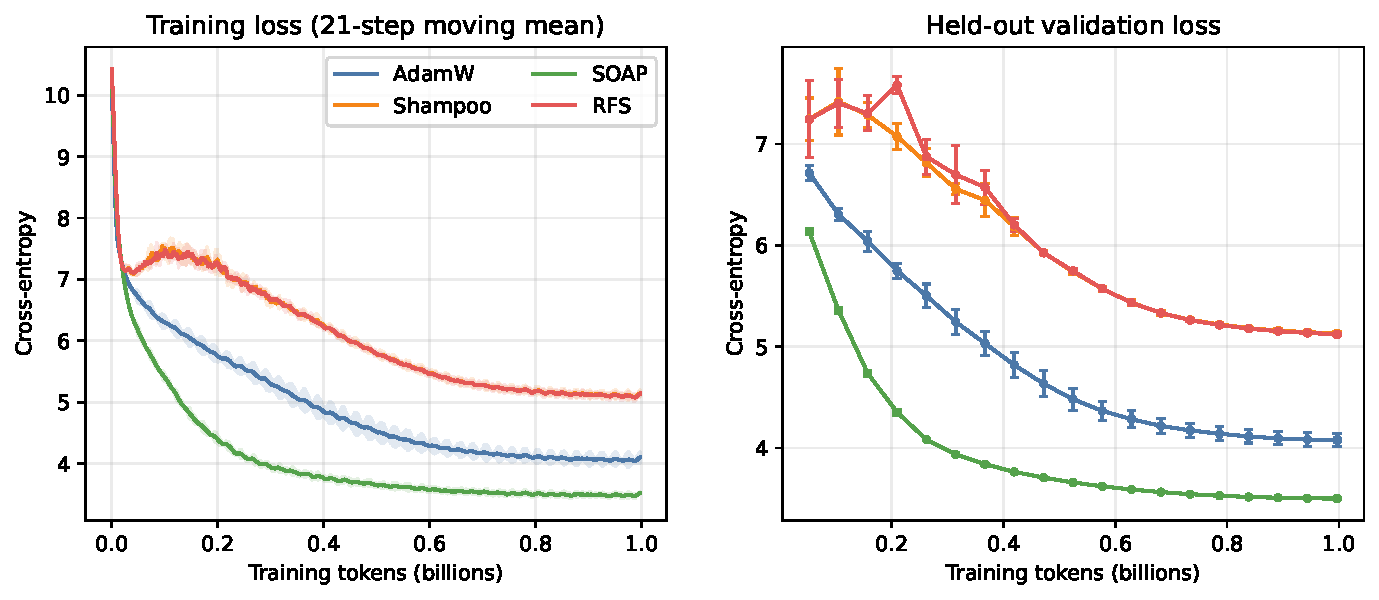
\includegraphics[width=\linewidth]{../figures/learning_curves.pdf}
  \caption{Training and held-out validation cross-entropy across three seeds.}
  \label{fig:curves}
\end{figure}

\begin{table}[t]
  \centering
  \caption{Final quality and systems measurements (mean $\pm$ sample standard
  deviation where shown).}
  \label{tab:results}
  \begin{tabular}{lrrrr}
\toprule
Optimizer & Test loss & Wall (h) & kTok/s & Peak GiB \\
\midrule
AdamW & 4.0515 $\pm$ 0.0671 & 0.798 & 351.5 & 38.7 \\
Shampoo & 5.1200 $\pm$ 0.0191 & 0.809 & 350.0 & 39.1 \\
SOAP & 3.4697 $\pm$ 0.0034 & 0.853 & 349.6 & 39.0 \\
RFS & 5.1123 $\pm$ 0.0081 & 0.816 & 350.1 & 39.1 \\
\bottomrule
\end{tabular}

\end{table}

\begin{figure}[t]
  \centering
  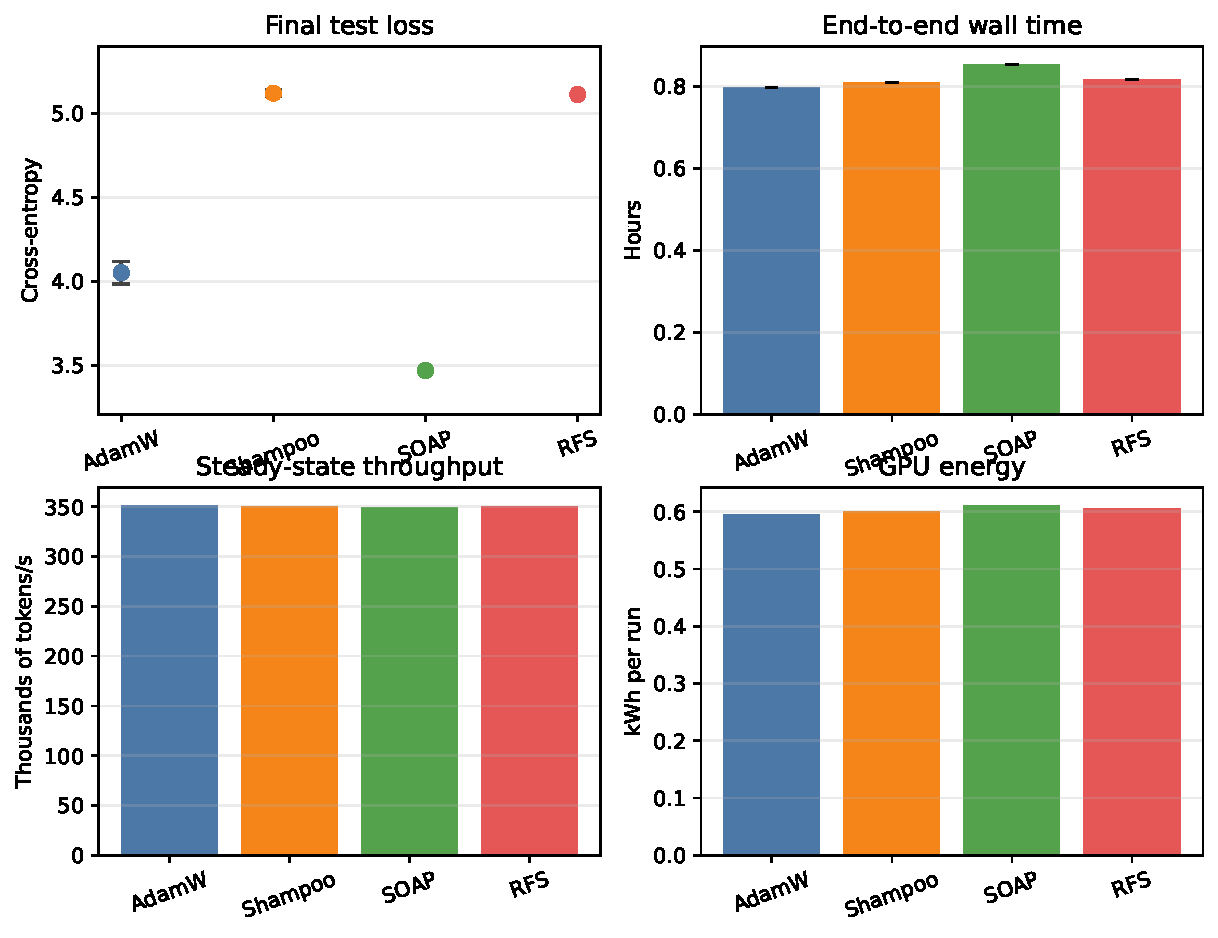
\includegraphics[width=\linewidth]{../figures/outcomes_and_systems.pdf}
  \caption{Final test loss, end-to-end wall time, and steady-state throughput.}
  \label{fig:systems}
\end{figure}

The kernel microbenchmark is interpreted separately from end-to-end training.
A faster elementwise primitive need not change total time when Transformer GEMMs
dominate, and a root refresh can be slower in isolation yet negligible at a long
refresh period. I therefore avoid extrapolating kernel speedups into optimizer
quality or total cost.

\section{Limitations}
The study covers one model scale, one corpus, one context length, and one accelerator.
Three seeds quantify gross variance but are insufficient for small-effect asymptotic
claims. Hyperparameter search is deliberately budgeted, so it cannot establish a
global optimum for any method. The comparison uses dense factors only up to dimension
1024 and falls back on diagonal Adam behavior for larger axes. Finally, the findings
concern the certified RFS realization tested here; other continuation or low-rank
\RFS{} engines may have different scaling.

\section{Reproducibility statement}
The repository records the source dataset revision and hashes, complete TOML/JSON
configuration, container base, host audit, native sources, unit tests, every JSONL
metric and telemetry sample, sweep decisions, three-seed summaries, figure-generation
code, and the time-varying cost ledger. Long runs begin only after corpus verification,
kernel parity, four-optimizer smoke tests, a full-model refresh test, and a finite
\RFS{} certificate.

\bibliographystyle{plainnat}
\bibliography{references}
\end{document}
